%!TEX TS-program = xelatex
\documentclass{EdipyLabs} % Custom class provided for EDIPY labs, by Christos Dalamagkas (cdalamagkas@gmail.com)
\SetLabNumber{5}
\SetLabTitle{Δρομολόγηση με το RIPv2}
\SetAuthor{Χρήστος Δαλαμάγκας}
\SetLabDescription{Δυναμική δρομολόγηση, πρωτόκολλα δρομολόγηση με διανύσματα απόσασης (distance-vector routing protocols), Router Information Protocol (RIP), RIPv2.}
\SetLabPrerequisites{Εργαστηριακά φυλλάδια 1β, 2α και 3 (Εισαγωγή στο RouterOS, Διευθέτηση δρομολογητή, Υποδικτύωση IPv4).}

\begin{document}
\Initialize

\section*{Εισαγωγή}
Αντικείμενο του παρόντος εργαστηριακού φυλλαδίου αποτελεί η εισαγωγή στη δυναμική δρομολόγηση με το πρωτόκολλο δρομολόγησης με διανύσματα απόστασης RIP. Η εργαστηριακή άσκηση αποτελείται από δυο σενάρια, το πρώτο αφορά τη βασική παραμετροποίηση του RIPv2 και το δεύτερο είναι ένα σενάριο επεκτασιμότητας, κατά το οποίο προσθέτετε έναν ακόμη δρομολογητή στην υπάρχουσα τοπολογία. Η τοπολογία που θα υλοποιήσετε στο πλαίσιο της εργαστηριακής άσκησης απεικονίζεται στο σχήμα \ref{fig:topology-generic}
\begin{figure}[ht]
	\centering
	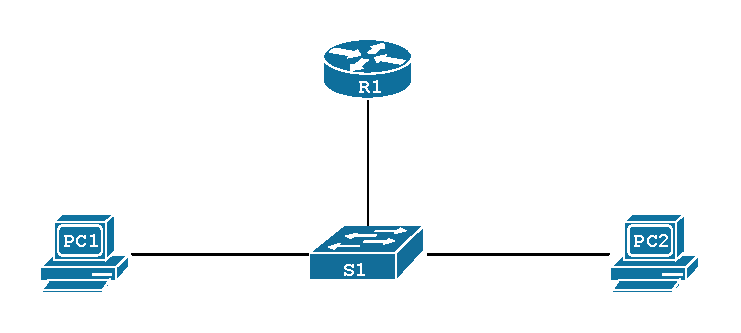
\includegraphics[width=\linewidth]{topology-generic}
	\caption{H γενική άποψη της τοπολογίας προς υλοποίηση}\label{fig:topology-generic}
\end{figure}

Για την υλοποίηση της τοπολογίας θα χρειαστείτε τις εξής συσκευές:
\begin{itemize}
	\item x2 δρομολογητές Cisco 2921
	\item x2 δρομολογητές MikroTik CCR-1009
	\item x2 μεταγωγείς Cisco Catalyst
	\item x4 υπολογιστές
\end{itemize}

\section{Θεωρητικό υπόβαθρο}
Στο προηγούμενο εργαστήριο είδατε πως ο διαχειριστής ενός δικτύου μπορεί να εισαγάγει χειροκίνητα κανόνες στατικής δρομολόγησης, ώστε να γνωστοποιήσει σε έναν δρομολογητή την ύπαρξη απομακρυσμένων δικτύων και να τον κατευθύνει για το ποια διεπαφή να χρησιμοποιήσει για να προωθήσει ένα πακέτο, ανάλογα με τον προορισμό του. Γίνεται αντιληπτό ότι η διαδικασία της χειροκίνητης ενημέρωσης των πινάκων δρομολόγησης γίνεται μη πρακτική για έναν διαχειριστή, όταν αυτός έχει υπό την επίβλεψη του ένα δίκτυο με πολλούς δρομολογητές και απομακρυσμένους προορισμούς.

Το ζήτημα της αυτοματοποιημένης ενημέρωσης των πινάκων δρομολόγησης αντιμετωπίζουν τα πρωτόκολλα δυναμικής δρομολόγησης. Ένα πρωτόκολλο δρομολόγησης προσδιορίζει το πως πρέπει να επικοινωνούν οι δρομολογητές μεταξύ τους, καθώς και τι είδους πληροφορίες ανταλλάσσουν, με σκοπό ο καθένας τους να είναι σε θέση να προωθήσει ένα πακέτο από την κατάλληλη διεπαφή, ώστε αυτό να φτάσει στον προορισμό του. Πολλά από αυτά τα πρωτόκολλα δημοσιεύονται σε έγγραφα RFC (Request for Comments), τα οποία είναι ελεύθερα διαθέσιμα, ώστε ο κάθε κατασκευαστής να τα υλοποιήσει για τους δικούς του δρομολογητές.

Όταν ενεργοποιηθεί ένα πρωτόκολλο δυναμικής δρομολόγησης σε ένα πλήθος δρομολογητών, επιτρέπει σε κάθε έναν από αυτούς να στείλει και να λάβει πληροφορίες, οι οποίες είναι γνωστές ως διαφημίσεις. Αυτή η ανταλλαγή διαφημίσεων έχει ως αποτέλεσμα, μετά από ένα χρονικό διάστημα, ο κάθε δρομολογητής να έχει πλήρη γνώση της δικτυακής τοπολογίας, έχοντας τη δυνατότητα να επικοινωνήσει με οποιοδήποτε απομακρυσμένο δίκτυο της τοπολογίας που έχει διαφημιστεί. Όταν όλοι οι δρομολογητές μιας τοπολογίας έχουν τις ίδιες τοπολογικές πληροφορίες, τότε το δίκτυο βρίσκεται σε \textbf{κατάσταση σύγκλισης} (convergance).

Μπορεί η δυναμική δρομολόγηση να παρέχει ευελιξία και να αποφορτίζει τους διαχειριστές, ωστόσο σε πραγματικές τοπολογίες η στατική δρομολόγηση συνυπάρχει με τη δυναμική. Οι βασικότεροι λόγοι συνύπαρξης της στατικής δρομολόγησης με τη δυναμική είναι διότι μια εφεδρική στατική διαδρομή με μεγαλύτερη διαχειριστική απόσταση (floating static route) μπορεί να ενεργοποιηθεί, αν τυχόν όλα τα δυναμικά πρωτόκολλα αποτύχουν. Ταυτόχρονα, η στατική δρομολόγηση είναι ιδανική για μικρής έκτασης δίκτυα, αφού δεν καταναλώνει ούτε εύρος ζώνης ούτε επεξεργαστικούς πόρους. Στον πίνακα \ref{tab:comparison} παρατίθενται τα συγκριτικά χαρακτηριστικά στατικής και δυναμικής δρομολόγησης.

\begin{table}[ht]\renewcommand\arraystretch{1.5}\rowcolors{2}{lightgray}{white}
\resizebox{\textwidth}{!}{
	\begin{tabular}{lll}\FormatFirstRow
										& \textbf{Δυναμική δρομολόγηση}						& \textbf{Στατική Δρομολόγηση}				\\
		\textbf{Περιπλοκότητα ρύθμισης}	& Γενικά ανεξάρτητη από το μέγεθος του δικτύου.		& Αυξάνεται με το μέγεθος του δικτύου.		\\
		\textbf{Ευελιξία}				& Αυτόματα προσαρμόζεται σε αλλαγές της τοπολογίας.	& Απαιτείται η παρέμβαση του διαχειριστή.	\\
		\textbf{Επεκτασιμότητα}			& Βολικό για απλές και για σύνθετες τοπολογίες.		& Βολική για απλές τοπολογίες.				\\
		\textbf{Ασφάλεια}				& Λιγότερο ασφαλής.									& Περισσότερο ασφαλής.						\\
		\textbf{Χρήση πόρων}			& Χρησιμοποιεί CPU, μνήμη, εύρος ζώνης.				& Δεν απαιτεί περαιτέρω πόρους.				\\
		\textbf{Προβλεψιμότητα}			& Η διαδρομή εξαρτάται από την τρέχουσα τοπολογία.	& Η διαδρομή προς τον προορισμό είναι πάντα η ίδια.
	\end{tabular}
}
\caption{Σύγκριση χαρακτηριστικών δυναμικής και στατικής δρομολόγησης.}\label{tab:comparison}
\end{table}

\subsection{Κατηγοριοποίηση πρωτοκόλλων δυναμικής δρομολόγησης}
Ένα από τα βασικότερα χαρακτηριστικά του Διαδικτύου είναι ότι διαθέτει ιεραρχική οργάνωση, με δεδομένη την έκτασή του, η οποία καλύπτει όλη την υφήλιο. Στο πλαίσιο της ιεραρχικής οργάνωσης έχουν υιοθετηθεί τα \textbf{Αυτόνομα Συστήματα} (Autonomous System - AS), δηλαδή ένα σύνολο από διευθύνσεις IP, οι οποίες ανήκουν σε έναν πάροχο ή διαχειριστική οντότητα, που εφαρμόζει συγκεκριμένους κανόνες για την πρόσβαση στο Διαδίκτυο και προς άλλες διαχειριστικές οντότητες.

Οι δρομολογητές που ανήκουν στο ίδιο αυτόνομο σύστημα χρησιμοποιούν πρωτόκολλα δρομολόγησης που ανήκουν στην κατηγορία των \textbf{Πρωτοκόλλων Εσωτερικής Πύλης} (Interior Gateway Protocols - IGP). Τα σημαντικότερα εξ αυτών είναι τα εξής: RIP, OSPF, EIGRP και IS-IS. 

Για την επικοινωνία δρομολογητών που ανήκουν σε διαφορετικά αυτόνομα συστήματα χρησιμοποιούνται \textbf{Πρωτόκολλα Εξωτερικής Πύλης} (Exterior Gateway Protocols - EGP), με το σημαντικότερο εξ αυτών το πρωτόκολλο BGP.

Πρόσθετα, τα πρωτόκολλα εσωτερικής πύλης διακρίνονται σε δρομολόγησης με \textbf{διανύσματα απόστασης} (distance-vector routing protocols), τα οποία κρίνουν τη βέλτιστη διαδρομή με βάση την απόσταση σε άλματα (hops) και διαφημίζουν διαδρομές, και τα πρωτόκολλα \textbf{κατάστασης συνδέσμων} (link-state routing protocols), τα οποία κρίνουν τη βέλτιστη διαδρομή με βάση το κόστος χρήσης/διάσχισης μιας σύνδεσης μεταξύ δυο κόμβων και διαφημίζουν καταστάσεις συνδέσμων.

\subsection{Το πρωτόκολλο RIP}
Το RIP (Routing Information Protocol) είναι ένα από τα παλαιότερα πρωτόκολλα δρομολόγησης, βασίζεται στους γνωστούς αλγορίθμους Bellman-Ford και Ford-Fulkerson, και ανήκει στην κατηγορία των πρωτοκόλλων δρομολόγησης με διανύσματα απόστασης εσωτερικής πύλης. Κυρίως, το πρωτόκολλο ορίζεται από τα έγγραφα \href{https://tools.ietf.org/html/rfc1058}{RFC 1058} (RIPv1), \href{https://tools.ietf.org/html/rfc2453}{RFC 2453} (RIPv2) και \href{https://tools.ietf.org/html/rfc2080}{RFC 2080} (RIPng για IPv6). 

Το μοναδικό κριτήριο του πρωτοκόλλου για την αξιολόγηση των διαδρομών είναι η απόσταση σε άλματα (hops). Μια διαδρομή ενός άλματος υποδηλώνει ένα απευθείας συνδεδεμένο δίκτυο, ενώ το μέγιστο πλήθος αλμάτων που υποστηρίζει ο αλγόριθμος είναι 15. Μια διαδρομή 16 αλμάτων υποδηλώνει μια μη διαθέσιμη διαδρομή (unreachable route). 

Για το IPv4 διακρίνονται δυο εκδόσεις του πρωτοκόλλου, το RIPv1 και το RIPv2. Σύμφωνα με την πρώτη έκδοση, ο δρομολογητής ευρυεκπέμπει κάθε 30 δευτερόλεπτα μια διαφήμιση με τον πίνακα δρομολόγησής του, από τις διεπαφές που έχει ενεργοποιηθεί το RIP. Το μήνυμα αυτό έχει ως προορισμό τη διεύθυνση περιορισμένης ευρυεκπομπής (limited broadcast) \ip{255.255.255.255}. Παράλληλα με τις ευρυεκπομπές, οι ενεργοποιημένες διεπαφές RIP ακούν για μηνύματα από άλλους δρομολογητές και όταν λάβουν μια διαφήμιση, στέλνουν τον δικό τους πίνακα δρομολόγησης ως απάντηση. 

Βασικό μειονέκτημα του RIPv1 είναι ότι οι μεταδιδόμενες ενημερώσεις δεν περιλαμβάνουν πληροφορίες σχετικά με τα προθέματα των δικτύων, συνεπώς, δεν μπορεί να υποστηριχθεί VLSM. Το κενό αυτό καλύπτεται από το RIPv2, το οποίο αντικαθιστά το RIPv1 και εντάσσει στις ενημερώσεις και τις αντίστοιχες μάσκες των δικτύων. Η δεύτερη έκδοση του πρωτοκόλλου αλλάζει τη διεύθυνση προορισμού των ενημερώσεων από ευρυεκπομπή στη διεύθυνση πολυδιανομής \ip{224.0.0.9} (multicast), ενώ προσθέτει δυνατότητα αυθεντικοποίησης των δρομολογητών RIPv2 μέσω MD5.

Το RIP διαθέτει ένα πλήθος από χρονόμετρα, τα οποία εξυπηρετούν στο να διατηρούνται ενημερωμένες οι διαδρομές στους πίνακες δρομολόγησης, ενώ ταυτόχρονα να μην επιβραδύνεται σοβαρά ο χρόνος σύγκλισης και το δίκτυο να μην κατακλύζεται από πολλές ενημερώσεις. Τα χρονόμετρα αυτά συνοψίζονται στα εξής:~
\begin{itemize}
	\item \textbf{update}: H περίοδος κατά την οποία το RIP ευρυεκπέμπει ή πολυδιανέμει τον πίνακα δρομολόγησης. Η προεπιλεγμένη τιμή είναι 30 δευτερόλεπτα.
	\item \textbf{invalid} ή \textbf{timeout}: Αν δεν ληφθεί ενημέρωση για μια διαδρομή μετά από αυτό το χρονικό διάστημα, τότε η διαδρομή θεωρείται λανθασμένη (invalid). Η προεπιλεγμένη τιμή είναι 180 δευτερόλεπτα.
	\item \textbf{hold down}: Για μια λανθασμένη διαδρομή, το χρονικό διάστημα κατά το οποίο απορρίπτονται ενημερώσεις με ίση ή χειρότερη μετρική. Το χρονόμετρο αυτό υπάρχει μόνο για τη Cisco. Η προεπιλεγμένη τιμή είναι 180 δευτερόλεπτα. 
	\item \textbf{flush} ή \textbf{garbage}: Μετά από αυτό το χρονικό διάστημα, μια λανθασμένη διαδρομή διαγράφεται από τον πίνακα δρομολόγησης. Η προεπιλεγμένη τιμή είναι 240 δευτερόλεπτα.
	
\end{itemize}

Το RIP, ως απλό πρωτόκολλο δρομολόγησης με διανύσματα απόστασης, δεν διατηρεί κάποια βάση δεδομένων/χάρτη της τοπολογίας, απλώς μαθαίνει και διαδίδει «φήμες» που αφορούν δίκτυα προορισμού. Αυτό το χαρακτηριστικό του, το κάνει ευάλωτο στη δημιουργία βρόχων δρομολόγησης (routing loops). Ένας βρόχος συμβαίνει όταν ένα πακέτο επιστρέφει σε έναν δρομολογητή από την ίδια ζεύξη. Το RIP υλοποιεί διάφορους μηχανισμούς για την αποτροπή των βρόχων:

\begin{itemize}
	\item \textbf{Μέγιστο πλήθος αλμάτων:} Τα 15 άλματα μέγιστης έκτασης της τοπολογίας ουσιαστικά εξυπηρετούν στο να αποτραπεί ένας βρόχος.
	\item \textbf{Split horizon:} Η μέθοδος απαγορεύει σε έναν δρομολογητή να προωθήσει τη διαφήμιση μιας περιοχής προς τη διεπαφή από την οποία την έλαβε.
	\item  \textbf{Route poisoning:} Ο δρομολογητής που μαθαίνει ότι μια διαδρομή είναι άκυρη (invalid), ενημερώνει όλους τους υπόλοιπους δρομολογητές για αυτό, αλλάζοντας το κόστος προς τη διαδρομή στο άπειρο (16 για το RIP).
	\item \textbf{Holddown}: Είναι το χρονόμετρο που περιγράφηκε προηγουμένως.
	\item \textbf{Triggered updates} (ενημερώσεις με έναυσμα): Ένας δρομολογητής RIP μπορεί άμεσα να στείλει ενημέρωση, όταν συνδέεται σε αυτόν ένα νέο δίκτυο, όταν μαθαίνει για ένα νέο δίκτυο, όταν αποσυνδέεται από αυτόν ένα δίκτυο ή όταν μαθαίνει ότι ένα δίκτυο είναι μη προσβάσιμο.
\end{itemize}

Παρόλο που στα σύγχρονα δικτυακά περιβάλλοντα το RIP δεν χρησιμοποιείται λόγω των χαμηλών επιδόσεων σε ταχύτητα σύγκλισης συγκριτικά με άλλα πρωτόκολλα IGP, ωστόσο αποτελεί σημαντικό για την εισαγωγή στη δυναμική δρομολόγηση λόγω της απλότητας του και της ευρύτατης υποστήριξης του ακόμη και από οικιακούς υπολογιστές και δρομολογητές.

\newpage

\section{Προετοιμασία δικτύου}

\begin{figure}[H]
	\centering
	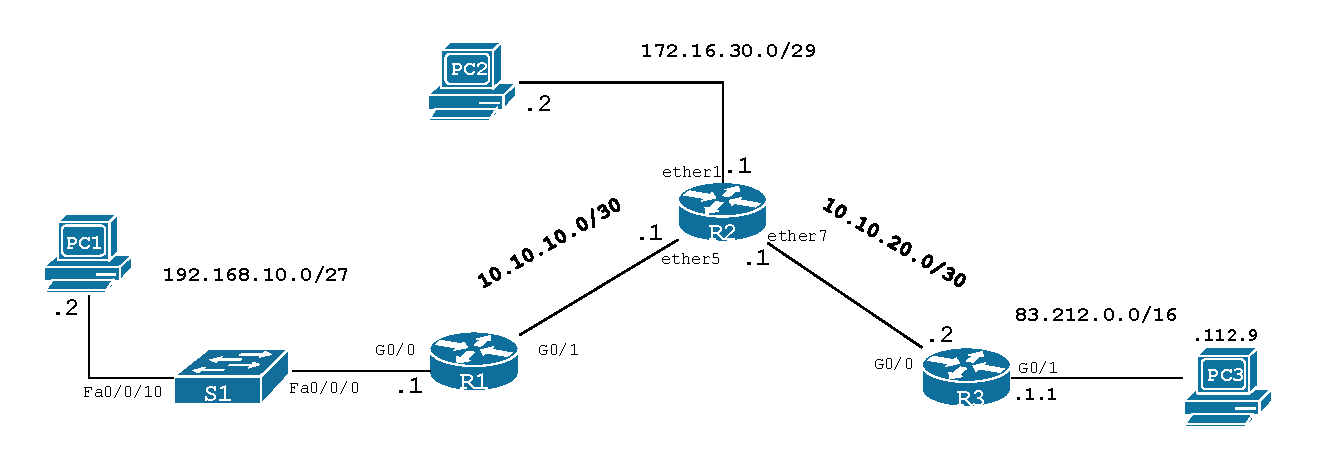
\includegraphics[width=\linewidth]{topology1}
	\caption{Το σχέδιο της αναλυτικής τοπολογίας προς υλοποίηση.}\label{fig:topology1}
\end{figure}

\begin{IpAddressTable}{Σχήμα διευθυνσιοδότησης της τοπολογίας του πρώτου σεναρίου.}{addr}
				 	 		 & Gi0/0		& 10.10.10.0	& 255.255.255.252		& 							  			\\	
\multirow{-2}{*}{R1}	 	 & Gi0/1		& 192.168.10.0	& 255.255.255.224		& \multirow{-2}{*}{-}		  			\\
\rowcolor{lightgray}	 	 & ether1		& 172.16.30.1	& 255.255.255.248		& 										\\
\rowcolor{lightgray}	 	 & ether5		& 10.10.10.1	& 255.255.255.252		& 										\\
\rowcolor{lightgray}
\multirow{-3}{*}{R2}		 & ether7		& 10.10.20.1	& 255.255.255.252		& \multirow{-2}{*}{-}					\\
						 	 & Gi0/0		& 10.10.20.2	& 255.255.255.252 		& 										\\
\multirow{-2}{*}{R3}		 & Gi0/1	  	& 83.212.1.1	& 255.255.0.0			& \multirow{-2}{*}{83.212.112.9}	\\
\rowcolor{lightgray}PC1 	 & \NIC	  		& 192.168.10.2	& 255.255.255.224 		& 192.168.10.1						\\
					PC2		 & \NIC	  		& 172.16.30.2	& 255.255.255.248		& 172.16.30.1						\\
\rowcolor{lightgray}PC3		 & \NIC	  		& 83.212.112.9	& 255.255.0.0			& 83.212.1.1						\\	
\end{IpAddressTable}

Ακολουθήστε τα εξής βήματα για την προετοιμασία του δικτύου της εργαστηριακής άσκησης:
\begin{itemize}
	\item Υλοποιήστε την συνδεσμολογία που απεικονίζεται στο σχήμα της τοπολογίας. Για το υπόλοιπο της άσκησης, θεωρείται πως ο δρομολογητής \textbf{MikroTik} είναι ο \textbf{R2}.
	\item Βεβαιωθείτε ότι όλες οι δικτυακές συσκευές λειτουργούν στις εργοστασιακές ρυθμίσεις.
	\item Αναθέστε διευθύνσεις IP στους υπολογιστές και τους δρομολογητές, σύμφωνα με το σχήμα διευθυνσιοδότησης.
	\item Αν κρίνετε ότι χρειάζεται, επιβεβαιώστε με την εντολή ping την σωστή παραμετροποίηση των διεπαφών για τις συνδέσεις σημείου προς σημείο.
\end{itemize}

\section{Σενάριο: Πρόσβαση στο «Διαδίκτυο»}
Στο συγκεκριμένο σενάριο θα ενεργοποιήσετε το πρωτόκολλο RIPv2 στους δρομολογητές, ώστε ο κάθε δρομολογητής να γνωστοποιεί τα δίκτυά του στους υπόλοιπους. Ακόμη, ο δρομολογητής R3 θα διαφημίσει την προεπιλεγμένη πύλη του, η οποία οδηγεί προς τον υπολογιστή R3, ο οποίος προσομοιώνει το Διαδίκτυο. Όλοι οι δρομολογητές της τοπολογίας πρέπει να χρησιμοποιούν ως προεπιλεγμένη πύλη τον κατάλληλο γειτονικό τους δρομολογητή ώστε να φτάσουν την προεπιλεγμένη πύλη του R3, δηλαδή τον PC3. 

\subsection{Παραμετροποίηση RIPv2 στον R1}
H ενεργοποίηση του πρωτοκόλλου RIP γίνεται με την είσοδο του διαχειριστή στην κατάσταση ρυθμίσεων \texttt{config-router} για το Cisco IOS. Εισέρχεστε στην κατάσταση αυτή με την εντολή \texttt{router rip} ως εξής:

\begin{CommandBox}
R1#`\textbf{conf t}`
R1(config)#`\textbf{router rip}`
R1(config-router)#
\end{CommandBox}

Από προεπιλογή, με την εντολή \texttt{router rip} τίθεται το RIPv1 σε λειτουργία. Για να ενεργοποιήστε το RIPv2 δώστε την εντολή \texttt{version~2}:

\begin{CommandBox}
R1(config-router)#`\textbf{version 2}`
\end{CommandBox}

Τα δίκτυα που θέλετε να διαφημίσετε μπορείτε να τα ορίσετε με την εντολή \texttt{network}, ακολουθούμενη από την ταυτότητα του δικτύου που θέλετε να διαφημίσετε. Ταυτόχρονα, με την εντολή αυτή ενεργοποιείτε το RIP στην αντίστοιχη διεπαφή που έχει το δίκτυο αυτό. Τα δίκτυα που πρέπει να διαφημίσει ο R1 προς τους υπόλοιπους δρομολογητές είναι τα \ip{192.168.10.0/27} και \ip{10.10.10.0/30}. Για να διαφημιστούν αυτά τα δίκτυα δώστε τις εντολές που ακολουθούν. Σημειώστε ότι στο Cisco IOS δεν χρειάζεται να συμπεριλάβετε τις μάσκες των δικτύων, αυτές ανακτώνται αυτόματα από τον πίνακα δρομολόγησης.

\begin{CommandBox}
R1(config-router)#`\textbf{network 192.168.10.0}`
R1(config-router)#`\textbf{network 10.10.10.0}`
\end{CommandBox}

Παρόλο που το RIPv2 υποστηρίζει VLSM, η υλοποίηση του πρωτοκόλλου από τη Cisco συναθροίζει τα δίκτυα στην ταξική τους μορφή, όπως το RIPv1. Συνεπώς, τα παραπάνω δίκτυα δεν έχουν μετατραπεί ακόμα σε αταξική μορφή, παρόλο που ενεργοποιήσατε το RIPv2. Για να απενεργοποιήσετε αυτή τη συμπεριφορά και να μετατρέψετε τα δίκτυα σε αταξική μορφή, απενεργοποιήστε την αυτόματη συνάθροιση με την εντολή \texttt{no auto-summary}:

\begin{CommandBox}
R1(config-router)#`\textbf{no auto-summary}`
\end{CommandBox}

Ενημερώσεις RIP στέλνονται από όλες εκείνες τις διεπαφές που έχουν ενεργοποιημένο το πρωτόκολλο RIP, οι οποίες έχουν έμμεσα δηλωθεί με την εντολή \texttt{network}. Για την περίπτωση του R1, ενημερώσεις στέλνονται από τις διεπαφές \texttt{G0/0} και \texttt{G0/1}. Ωστόσο, διαπιστώνει κάποιος ότι δεν χρειάζεται να στέλνονται ενημερώσεις μέσω της διεπαφής \texttt{G0/0}, η οποία επικοινωνεί με το LAN, αφού δεν υπάρχει εκεί κάποιος δρομολογητής ο οποίος μπορεί να αξιοποιήσει τα μηνύματα αυτά. Συνήθης πρακτική είναι να αποτρέπεται η αποστολή ενημερώσεων μέσω των διεπαφών που δεν επικοινωνούν με δρομολογητές RIP, ορίζοντάς τες ως παθητικές, με την εντολή \texttt{passive-interface} ακολουθούμενη από τον αριθμό της διεπαφής. Για τον R1, ορίστε τη διεπαφή που επικοινωνεί με το LAN ως παθητική με την ακόλουθη εντολή:

\begin{CommandBox}
R1(config-router)#`\textbf{passive-interface g0/0}`
\end{CommandBox}

Μπορείτε να επιβεβαιώσετε τις ρυθμίσεις πρωτοκόλλων δυναμικής δρομολόγησης που έχουν εφαρμοστεί με την εντολή \texttt{show ip protocols}

\begin{CommandBox}
R1#`\textbf{show ip protocols}`
\end{CommandBox}

\subsection{Παραμετροποίηση RIPv2 στον R2}
Η ρύθμιση του πρωτοκόλλου RIP στο RouterOS γίνεται από τον υποκατάλογο \texttt{/routing rip}. Η ρύθμιση RIP απαιτεί ως πρώτο βήμα την ενεργοποίηση του πρωτοκόλλου για τις διεπαφές, των οποίων τα δίκτυα θέλουμε να διαφημίσουμε. Οι διεπαφές αυτές είναι οι \texttt{ether1}, \texttt{ether5} και \texttt{ether7}, οι οποίες ρυθμίζονται με τις εντολές που ακολουθούν. Επισημαίνεται ότι το RοuterOS από προεπιλογή στέλνει τις ενημερώσεις σε RIPv2. Ακόμη, η διεπαφή \texttt{ether1} τίθεται σε παθητική κατάσταση, αφού συνδέεται απευθείας με το LAN. 

\begin{CommandBox}
[admin@R2] > `\textbf{routing rip interface}`
[admin@R2] routing rip interface > `\textbf{add interface=ether1 passive=yes}`
[admin@R2] routing rip interface > `\textbf{add interface=ether5}`
[admin@R2] routing rip interface > `\textbf{add interface=ether7}`
\end{CommandBox}

Στη συνέχεια, πρέπει να ορίσετε τα δίκτυα που θέλετε να διαφημίσετε μέσω του υποκαταλόγου \texttt{routing rip network}. Για να διαφημίσετε τα τρία δίκτυα του R2 δώστε τις εντολές που ακολουθούν. Προσέξτε ότι μαζί με τις ταυτότητες των δικτύων πρέπει να συμπεριλάβετε και το αντίστοιχο μήκος προθέματος.

\begin{CommandBox}
[admin@R2] routing rip interface > `\textbf{.. network}`
[admin@R2] routing rip network > `\textbf{add network=10.10.10.0/30}`
[admin@R2] routing rip network > `\textbf{add network=172.16.20.0/29}`
[admin@R2] routing rip network > `\textbf{add network=10.10.20.0/30}`
\end{CommandBox}

\subsection{Παραμετροποίηση RIPv2 στον R3}
Δώστε τις κατάλληλες εντολές στον R3 ώστε να διαφημίσετε το δίκτυο σημείου-προς-σημείο που συνδέει απευθείας τον R3 με τον R2. \textbf{MHN} διαφημίσετε το δίκτυο του PC3, διότι αυτό προσομοιώνει το Διαδίκτυο.

Πρόσθετη δυνατότητα ενός πρωτοκόλλου δυναμικής δρομολόγησης είναι να διαφημίζει την προεπιλεγμένη πύλη του πίνακα δρομολόγησης, ώστε αυτή να υιοθετείται από τους υπόλοιπους δρομολογητές της τοπολογίας. 
Αποτέλεσμα της διάδοσης αυτής είναι ότι κάθε πακέτο που προέρχεται από οποιονδήποτε δρομολογητή και έχει άγνωστο προορισμό, να προωθείται προς την προεπιλεγμένη πύλη του δρομολογητή που διαφημίζει την προεπιλεγμένη πύλη του. Για την περίπτωση του R3, κάθε πακέτο που προορίζεται προς οποιονδήποτε άγνωστο προορισμό, πρέπει να προωθείται στον υπολογιστή R3, ο οποίος προσομοιώνει την πρόσβαση στο Διαδίκτυο. Για να ενεργοποιήσετε τη διάδοση της προεπιλεγμένης πύλης από τον R3 δώστε την εντολή \texttt{default-information originate}:

\begin{CommandBox}
R1(config-router)#`\textbf{default-information originate}`
\end{CommandBox}

\subsection{Δοκιμές συνδεσιμότητας}
Αφού ρυθμίσετε το RIPv2 σε όλους τους δρομολογητές, περιμένετε μερικά δευτερόλεπτα, αν χρειαστεί, ώστε το δίκτυο να συγκλίνει. Παρατηρήστε τους πίνακες δρομολόγησης κάθε δρομολογητή για να επιβεβαιώσετε ότι οι εγγραφές είναι σωστές. 

Στον R3 πρέπει να δείτε όλα τα απομακρυσμένα δίκτυα που έχετε διαφημίσει, δηλαδή τα LAN των R1 και R2, καθώς και το δίκτυο σημείου προς σημείο του R1 με τον R2.
\begin{CommandBox}
R3#`\textbf{show ip route | begin Gateway}`
Gateway of last resort is 83.212.112.9 to network 0.0.0.0

	192.168.10.0/27 is subnetted, 1 subnets
`\hl{R}`	  `\hl{192.168.10.0 [120/2] via 10.10.20.1, 00:00:16, GigabitEthernet0/0}`
	83.0.0.0/16 is subnetted, 1 subnets
C	  83.212.0.0 is directly connected, GigabitEthernet0/1
	172.16.0.0/29 is subnetted, 1 subnets
`\hl{R}`	  `\hl{172.16.30.0 [120/1] via 10.10.20.1, 00:00:16, GigabitEthernet0/0}`
	10.0.0.0/30 is subnetted, 2 subnets
`\hl{R}`	  `\hl{10.10.10.0 [120/1] via 10.10.20.1, 00:00:16, GigabitEthernet0/0}`
C	10.10.20.0 is directly connected, GigabitEthernet0/0
S*  0.0.0.0/0 [1/0] via 83.212.112.9
R3#
\end{CommandBox}

Ο πίνακας δρομολόγησης για τον R2 παρατίθεται παρακάτω. Διακρίνεται το επόμενο άλμα που χρειάζεται για να προσεγγισθεί η πύλη δικτύου του R3, δηλαδή ο R3 με διεύθυνση \ip{10.10.20.2}, ως πύλη δικτύου του R2, καθώς και το LAN του R1, ως απομακρυσμένο δίκτυο.

\begin{CommandBox}
[admin@R2] > `\textbf{ip route print}`
`\begin{tabular}{llllll}
	\#&   &   DST-ADDRESS&        PREF-SRC&        GATEWAY&            DISTANCE\\
	\hl{0}& \hl{ADr}&  \hl{0.0.0.0/0}&                   &       \hl{10.10.20.2}&              \hl{120}\\
	1& ADC&  10.10.10.0/30&      10.10.10.1&      ether2&                    0\\		
	2& ADC&  10.10.20.0/30&      10.10.20.1&      ether3&                    0\\
	3& ADC&  172.16.30.0/29&     172.16.30.1&     ether1&                    0\\
	\hl{4}& \hl{ADr}&  \hl{192.168.10.0/27}&               &     \hl{10.10.10.2}&              \hl{120}
\end{tabular}`
[admin@MikroTik] >
\end{CommandBox}

Τέλος, ο πίνακας δρομολόγησης του R1 πρέπει να έχει ως πύλη δικτύου το επόμενο άλμα για να προσεγγιστεί η πύλη δικτύου του R3, δηλαδή τον R2 με διεύθυνση  \ip{10.10.10.1}, το απομακρυσμένο LAN του R2, καθώς και η δίκτυο σημείου προς σημείο του R2 με τον R3.

\begin{CommandBox}
R1#`\textbf{show ip route | begin Gateway}`
`\hl{Gateway of last resort is 10.10.10.1 to network 0.0.0.0}`
	
	192.168.10.0/27 is subnetted, 1 subnets
C	  192.168.10.0 is directly connected, GigabitEthernet0/0
	172.16.0.0/29 is subnetted, 1 subnets
`\hl{R}`	  `\hl{172.16.30.0 [120/1] via 10.10.10.1, 00:00:23, GigabitEthernet0/1}`
	10.0.0.0/30 is subnetted, 2 subnets
C	   10.10.10.0 is directly connected, GigabitEthernet0/1
`\hl{R}`    `\hl{10.10.20.0 [120/1] via 10.10.10.1, 00:00:23, GigabitEthernet0/1}`
`\hl{R*}`   `\hl{0.0.0.0/0 [120/2] via 10.10.10.1, 00:00:23, GigabitEthernet0/1}`
R1#
\end{CommandBox}

Από τους υπολογιστές PC1 και PC2 κάντε \ip{ping} στη διεύθυνση \ip{83.212.112.9} του PC3. Η διεύθυνση αυτή προσομοιώνει το Διαδίκτυο, αφού είναι άγνωστη στους ενδιάμεσους δρομολογητές, με αποτέλεσμα ο κάθε δρομολογητής να χρησιμοποιεί την πύλη δικτύου που διαφημίστηκε από τον R3. Θα πρέπει τα πακέτα ICMP να σταλούν και να επιστρέψουν με επιτυχία.

Αν αντιμετωπίσετε προβλήματα συνδεσιμότητας ή διαπιστώσετε πως οι πίνακες δρομολόγησης δεν έχουν τα σωστά περιεχόμενα, τότε ακολουθήστε τα βήματα της ενότητας «Αντιμετώπιση Προβλημάτων».
\newpage

\section{Σενάριο: Επεκτασιμότητα με το RIPv2}
Τροποποιήστε την τοπολογία, συνδέοντας έναν νέο δρομολογητή σε μια ελεύθερη διεπαφή του R1. H τοπολογία και ο πίνακας διευθυνσιοδότησης λαμβάνουν την εξής μορφή:

\begin{figure}[H]
	\centering
	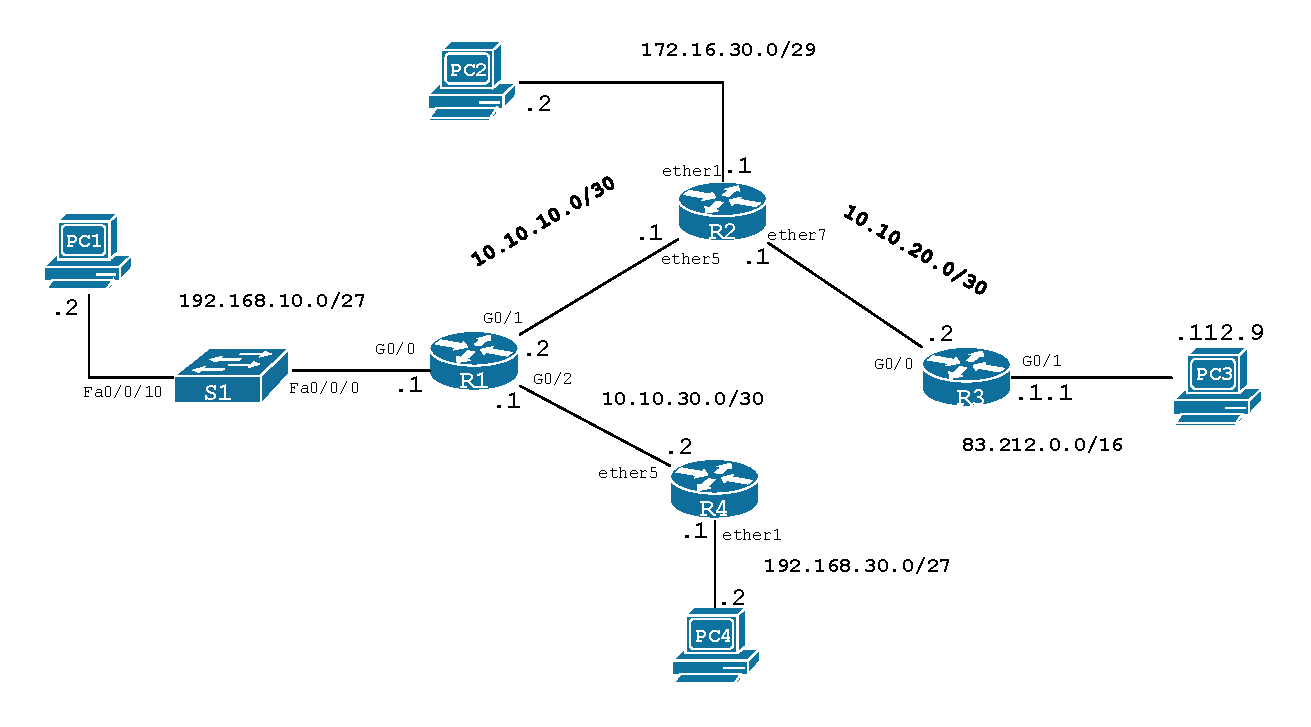
\includegraphics[width=\linewidth]{topology2}
	\caption{Το σχέδιο της αναλυτικής τοπολογίας προς υλοποίηση.}\label{fig:topology2}
\end{figure}

\begin{IpAddressTable}{Σχήμα διευθυνσιοδότησης της τοπολογίας του δεύτερου σεναρίου.}{addr2}
	R1				 & Gi0/2		& 10.10.30.1			& 255.255.255.252 		& -					\\	
\rowcolor{lightgray}
				 	 & ether5		& 10.10.30.2			& 255.255.255.252 		& 					 \\
\rowcolor{lightgray}	
\multirow{-2}{*}{R4} & ether1		& 10.10.20.1	 		& 255.255.255.252 		& \multirow{-2}{*}{-} \\
PC4  				 & \NIC	  		& 192.168.30.2			& 255.255.255.224 		& 192.168.30.1
\end{IpAddressTable}

Αφού εφαρμόσετε τις νέες ρυθμίσεις διευθυνσιοδότησης που φαίνονται στον πίνακα \ref{tab:addr2}, εφαρμόστε τις παραμετροποιήσεις RIPv2 που κρίνετε απαραίτητες ώστε ο PC4 να επικοινωνήσει με τον PC3.
\newpage

\section{Αντιμετώπιση προβλημάτων με το RIP}
Αν αντιμετωπίζετε προβλήματα συνδεσιμότητας ακολουθήστε τα εξής βήματα, ξεκινώντας από τα χαμηλότερα στρώματα του OSI και καταλήγοντας στο επίπεδο δικτύου, όπου βρίσκονται τα πρωτόκολλα δυναμικής δρομολόγησης.
\begin{itemize}
	\item Βεβαιωθείτε ότι οι φωτεινές ενδείξεις στις φυσικές θύρες είναι πράσινες και με τις κατάλληλες εντολές επιβεβαιώστε τις σωστές ρυθμίσεις IP. Aν είναι αναγκαίο, κάντε \ip{ping} μεταξύ των συσκευών που συνδέονται απευθείας ώστε να επιβεβαιώσετε ότι εφαρμόσατε τις σωστές ρυθμίσεις IP.
	\item Προβάλλετε τους πίνακες δρομολόγησης της κάθε συσκευής. Αν δεν βλέπετε δυναμικές καταχωρήσεις από το πρωτόκολλο RIP, τότε σημαίνει πως δεν διαδίδονται σωστά οι διαδρομές.
	\item Για να επαναφέρετε το πρωτόκολλο RIP σε έναν δρομολογητή Cisco δώστε την εντολή:
\begin{CommandBox}
Router(config)#`\textbf{no router rip}`
\end{CommandBox}
	Για τους δρομολογητές MikroTik διαγράψτε όλα τα αντικείμενα από τις λίστες \texttt{/routing rip network} και \texttt{routing rip interface}. 
	\item Όσο είναι σε λειτουργία το RIP μπορείτε να προβάλλετε χρήσιμες πληροφορίες σχετικά με γεγονότα που συμβαίνουν (λήψεις/αποστολές μηνυμάτων) και σχετίζονται με το RIP. Για τους δρομολογητές Cisco μπορείτε να δώσετε την εξής εντολή ώστε να ενεργοποιήσετε την εμφάνιση των μηνυμάτων: 
\begin{CommandBox}
Router#`\textbf{debug ip rip}`
\end{CommandBox}
	Η απενεργοποίηση της αποσφαλμάτωσης μπορεί να γίνει με την εντολή \texttt{no debug ip rip} ή την εντολή:
\begin{CommandBox}
Router#`\textbf{undebug all}`
\end{CommandBox}
	Για τους δρομολογητές MikroTik, μπορείτε να ανατρέξετε στον κατάλογο \texttt{/log} και με την εντολή \ip{print} να προβάλλετε όλες οι καταγραφές από όλες τις υπηρεσίες του RouterOS. Για να βλέπετε ασύγχρονα τα μηνύματα που σχετίζονται με το πρωτόκολλο RIP δώστε την εντολή:		
\begin{CommandBox}
[admin@MikroTik] > `\textbf{log print follow where topics=rip}`
\end{CommandBox}
	
\end{itemize}

\end{document}
